




\section{Introduction} 


\section{Queueing Theory}

\begin{frame}
    \frametitle{Introduction}

    Queueing theory is the theory behind what happens when you have
    lots of jobs, scarce resources, and subsequently long queues and delays.
    The goals of queueing theorist are:

    \begin{itemize}
        \item \textbf{Predicting the system performance:} Tipically this means predicting mean delay or the 
        probability that delay exceeds some Service Level Agreement (SLA);
        
        \item \textbf{Finding a superior system design:} Determines which additional resources, smarter 
        scheduling, others.
    \end{itemize}


\end{frame}


\begin{frame}
    \frametitle{The Single-Server Network}

    Queueing network is made up servers

    \begin{itemize}
        \item \textbf{Service Order:} The order in which jobs will be served by 
        the server (First-Come-First-Served - FCFS);

        \item \textbf{Average Arrival Rate ($\lambda$):} This is the average at which job arrive
        to the server (e.g., $\lambda = 3 jobs/sec$);

        \item \textbf{Mean Interarrival Time:}  Average time between successive job
        arrivals (e.g., $1/\lambda = 1/3 sec$);

        \item \textbf{Service Requirement, Size:} The job time. Tipically denoted by 
        the random variable $S$;

        \item \textbf{Mean Service Time:} This is the expected value of $S$ ($\E[S]$)

        \item \textbf{Average Service Rate ($\mu$):} This is the average rate at which job 
        are served (e.e, $\mu = 4 jobs/sec = 1/E[S]$)
    \end{itemize}

\end{frame}



\begin{frame}
    \frametitle{The Single-Server Network: Performance Metrics}

    Queueing network is made up servers

    \begin{itemize}
        \item \textbf{Response Time ($T$)} Is givev by:

        $$T = t_{depart} - t_{arrive}$$

        Where $t_{depart}$ is the time when the job leaves the system, and $t_{arrive}$ is the
        time when the job arrive. {\color{red}Where are interested in $E[T]$ and $Var[T]$}

        \item \textbf{Waiting Time or Delay ($T_Q$):} This is the time that the job spends in 
        the queue (wasted time).

        \item \textbf{Number of Jobs in the System ($N$):}  Includes jobs in the queue plus into 
        the server;

        \item \textbf{Number if jobs in the Queue ($N_Q$):} Number of jobs waiting in the queue.

    \end{itemize}

\end{frame}



\begin{frame}
    \frametitle{The Single-Server Network: More Metrics}

    \begin{itemize}
       
        
        \item \textbf{Utilization ($\rho$):} Is the fraction of time is busy. Let $\tau$ denote
        the length of the observation period. Let $B$ denote the total time
        during the observation period that the device {\color{red}is busy}. Then 

        $$\rho = \frac{B}{\tau}$$
      
        \item \textbf{Throughput ($X$):} Is the rate of completions at device (e.g., jobs/sec);
        Let $C$ denote the total number of jobs {\color{red}completed} at 
        device during time $\tau$. Then

        $$X = \frac{C}{\tau}$$


    \end{itemize}

\end{frame}



\begin{frame}
    \frametitle{The Single-Server Network: More Metrics}

    So how does $X$ related to $\rho$?

    $$X = \frac{C}{B}\rho$$

    Where $C/B$ is:

    $$\frac{C}{B} = \frac{\text{Number of Completed (jobs)}}{\text{Time is busy (sec)}} 
    = E[S] \Rightarrow {\color{red}E[S] = \frac{1}{\mu}}$$

    Finally:

    $$X = \mu \rho$$
   
\end{frame}



\begin{frame}
    \frametitle{The Single-Server Network}

    \begin{figure}
        \centering
        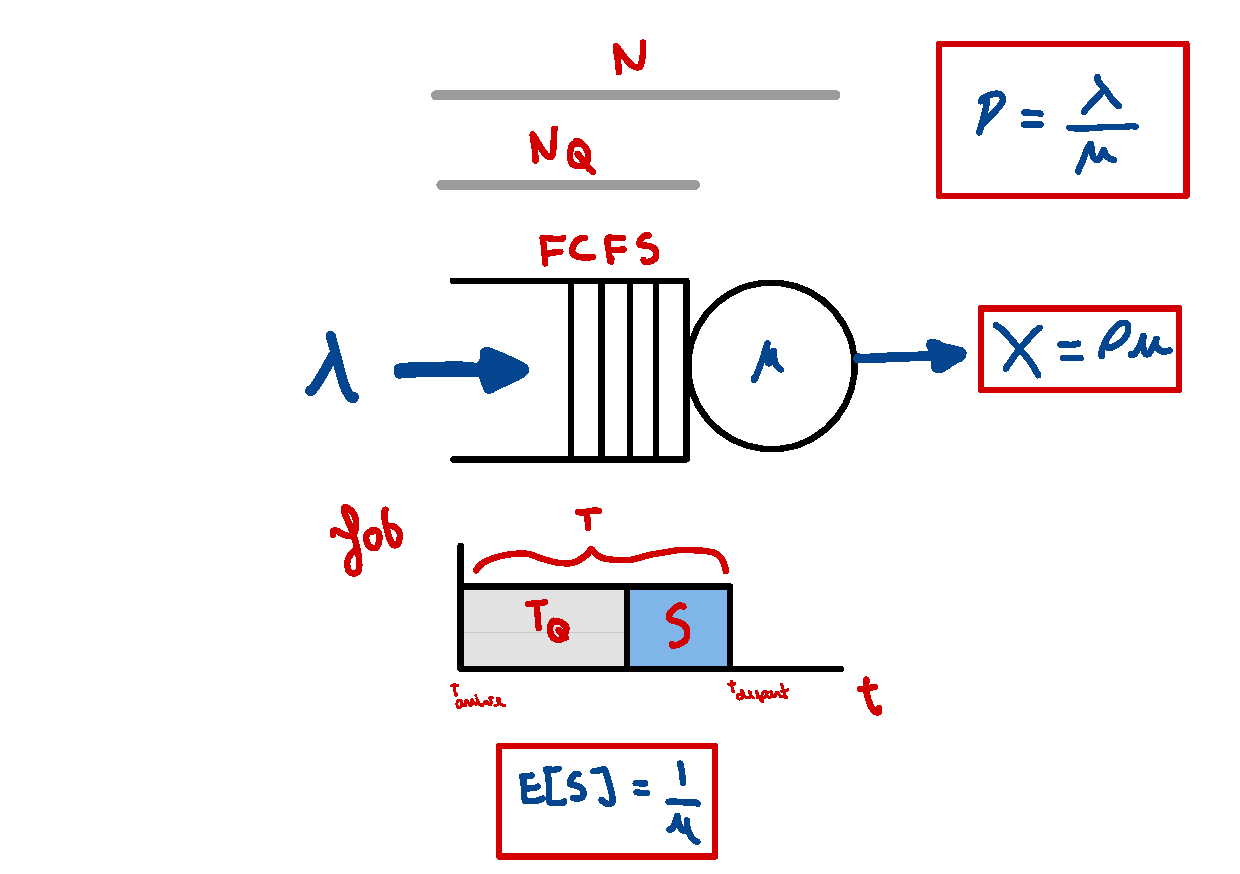
\includegraphics[width=0.95\textwidth]{slides/figures/simple_queue_example.pdf}
    \end{figure}

\end{frame}



\begin{frame}
    \frametitle{Classification of Queueing Networks}

    Queueing networks can be classified into two categories:

    \begin{itemize}
       \item \textbf{Open networks:} receive customers from an external
       source and send them to an external destination;

       \item \textbf{Closed networks:} have a fixed population that moves between 
       the queues but never leaves the system.
    \end{itemize}

\end{frame}



\begin{frame}
    \frametitle{Open Networks}
    \begin{figure}
        \centering
        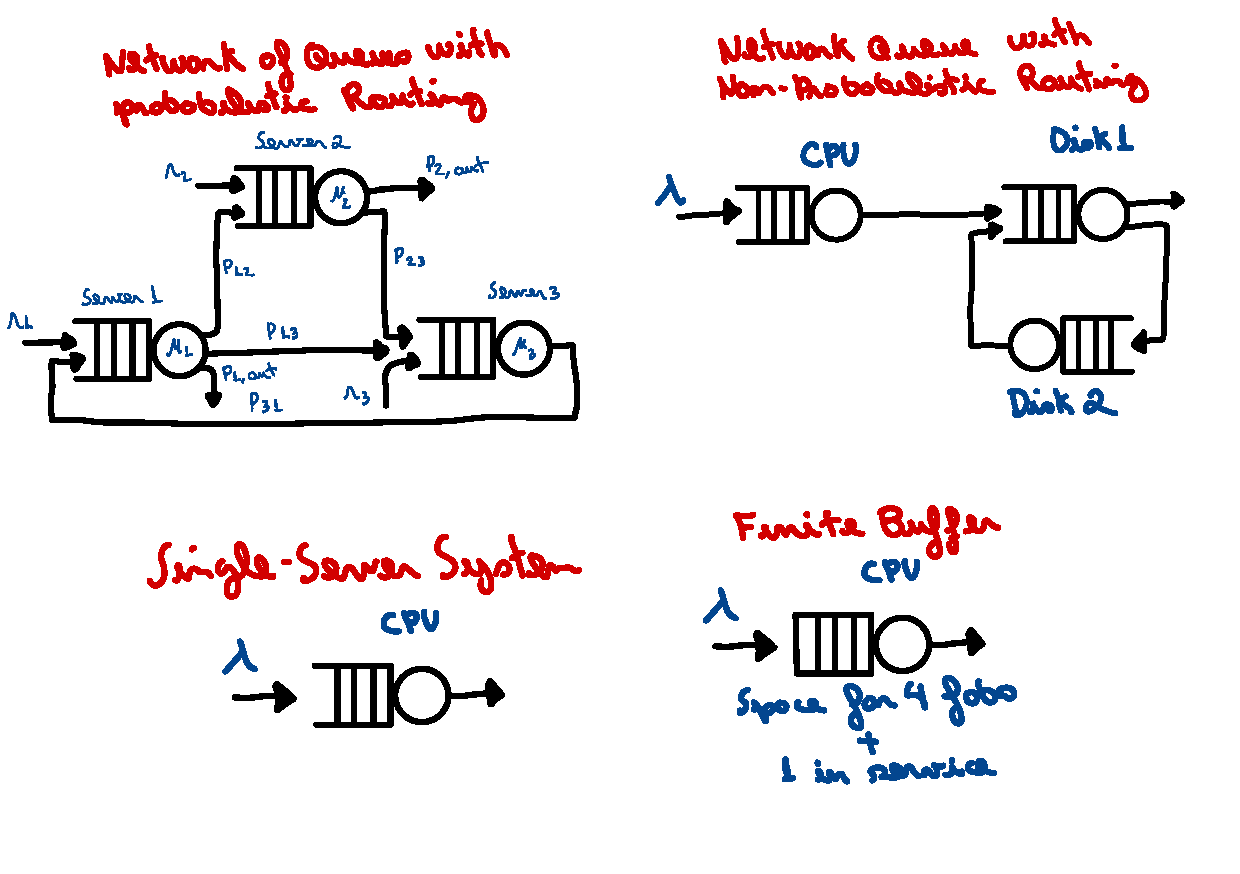
\includegraphics[width=0.95\textwidth]{slides/figures/open_networks_example.pdf}
    \end{figure}
\end{frame}




\begin{frame}
    \frametitle{Closed Networks}

    Closed queueing networks have no external arrivals or departures. 
    They can be classified into two categories:

    \begin{itemize}
       \item \textbf{Interactive:} receive customers from an external
       source and send them to an external destination;

       \item \textbf{Batch system:} have a fixed population that moves between 
       the queues but never leaves the system.
    \end{itemize}

\end{frame}


\subsection{Little's Law}


\begin{frame}
    \frametitle{Little's Law for Open Systems}

    \begin{definition}
        For any ergodic open system we have that
        $$E[N] = \lambda E[T]$$

        where $E[N]$ is the expected number of jobs in the system, $\lambda$
        is the average arrival rate into the system, and $E[T]$ is the 
        mean time jobs spend in the system
    \end{definition}

\end{frame}



\begin{frame}
    \frametitle{Little's Law for Open Systems (Intuition)}

    
    \begin{itemize}

        \item It should seem intuitive that $E[T]$ and $E[N]$ are proportinal!

        \item Consider a fast-food restaurant: It gets people out fast (low $E[T]$)
        and also does not require much waiting room (low $E[N]$);

        \item By contrast, a slow-service restaurant gets people out slowly 
        (high $E[T]$) and therefore needs a lot more seating room ($E[N]$);


    \end{itemize}

\end{frame}


%\begin{frame}
%    \frametitle{Little's Law for Open Systems (Intuition)}
%    \begin{figure}
%        \centering
%        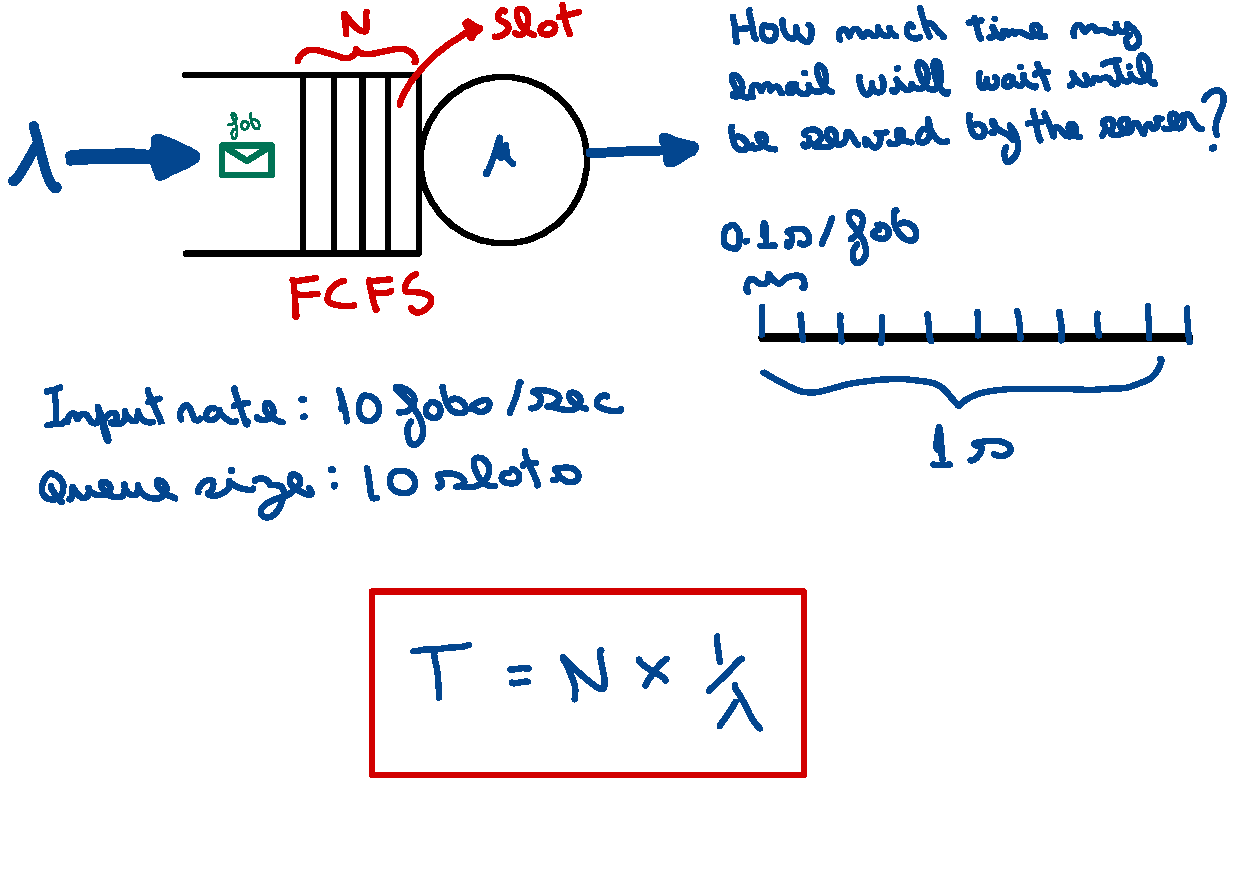
\includegraphics[width=0.95\textwidth]{slides/figures/little_law_open_network_intuition.pdf}
%    \end{figure}
%\end{frame}


\begin{frame}
    \frametitle{Little's Law for Open Systems (Proof)}

    
    \begin{itemize}

        \item As you see, Little's Law is actually stated as a relationship
        between time averages. Let

        $$\lambda = \lim_{t \to\infty} \frac{A(t)}{t} \text{~~and~~} X = lim_{t \to\infty} \frac{C(t)}{t},$$

        where $A(T)$ is the number of arrivals by time $t$ abd $C(t)$ is the number
        of system competions (departures);

        \item Tipically {\color{red}$\lambda=X$} (input rate is equal than output rate);

    \end{itemize}

\end{frame}



\begin{frame}
    \frametitle{Little's Law for Open Systems (Proof)}

    
    \begin{figure}
        \centering
        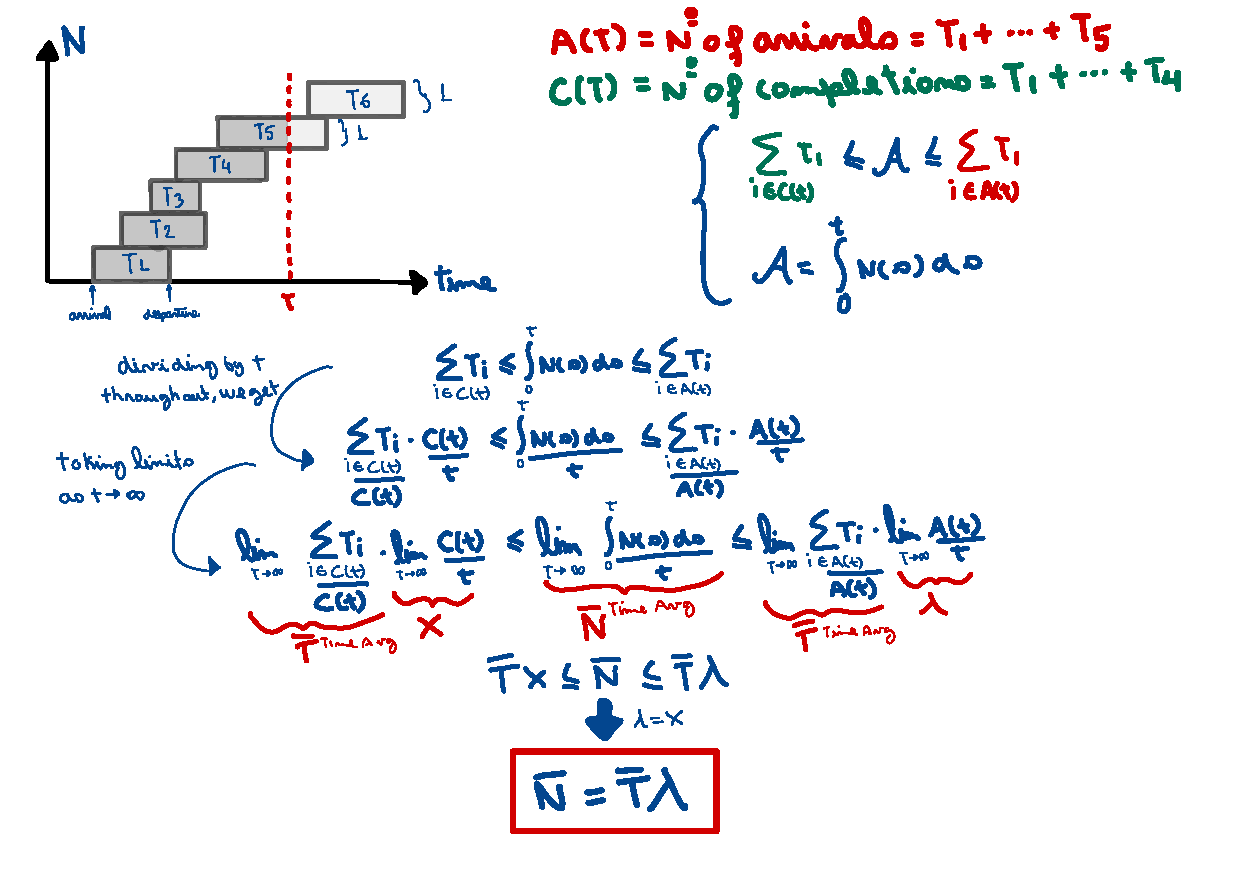
\includegraphics[width=0.95\textwidth]{slides/figures/little_law_open_proof.pdf}
    \end{figure}

\end{frame}



\begin{frame}
    \frametitle{Little's Law for Closed Systems}

    \begin{definition}
        Given any ergodic closed systems,

        $$N = X E[T]$$

        where $N$ is a constant equal to the multiprogramming level, $X$
        is the throughput (i.e, the rate of competions for the system),
        $E[T]$ is the mean time jobs spend in the system, and $\lambda=X$.

    \end{definition}

\end{frame}

\begin{frame}
    \frametitle{Little's Law for Closed Systems (Proof)}
    \begin{figure}
        \centering
        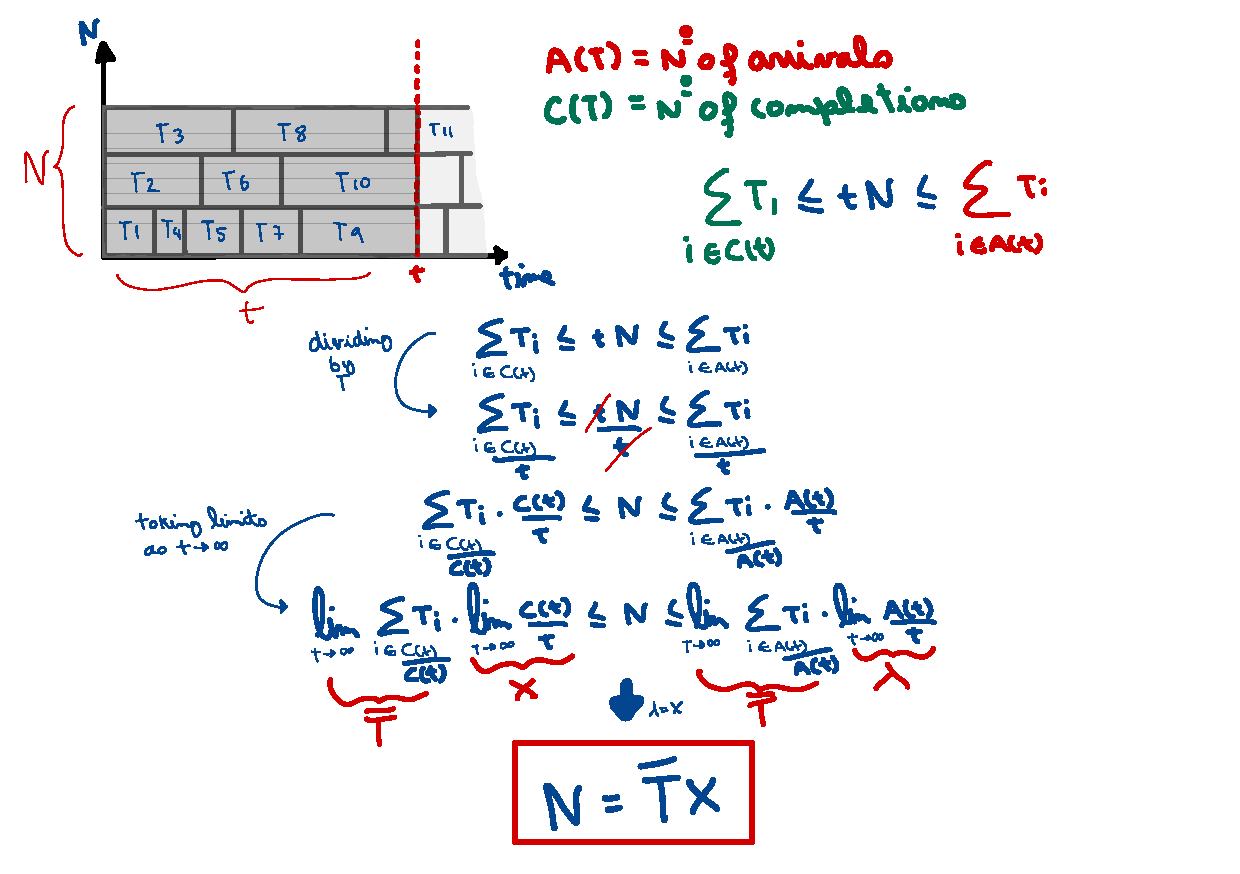
\includegraphics[width=0.95\textwidth]{slides/figures/little_law_closed_proof.pdf}
    \end{figure}
\end{frame}



\begin{frame}
    \frametitle{Little's Law: Example}
    \begin{figure}
        \centering
        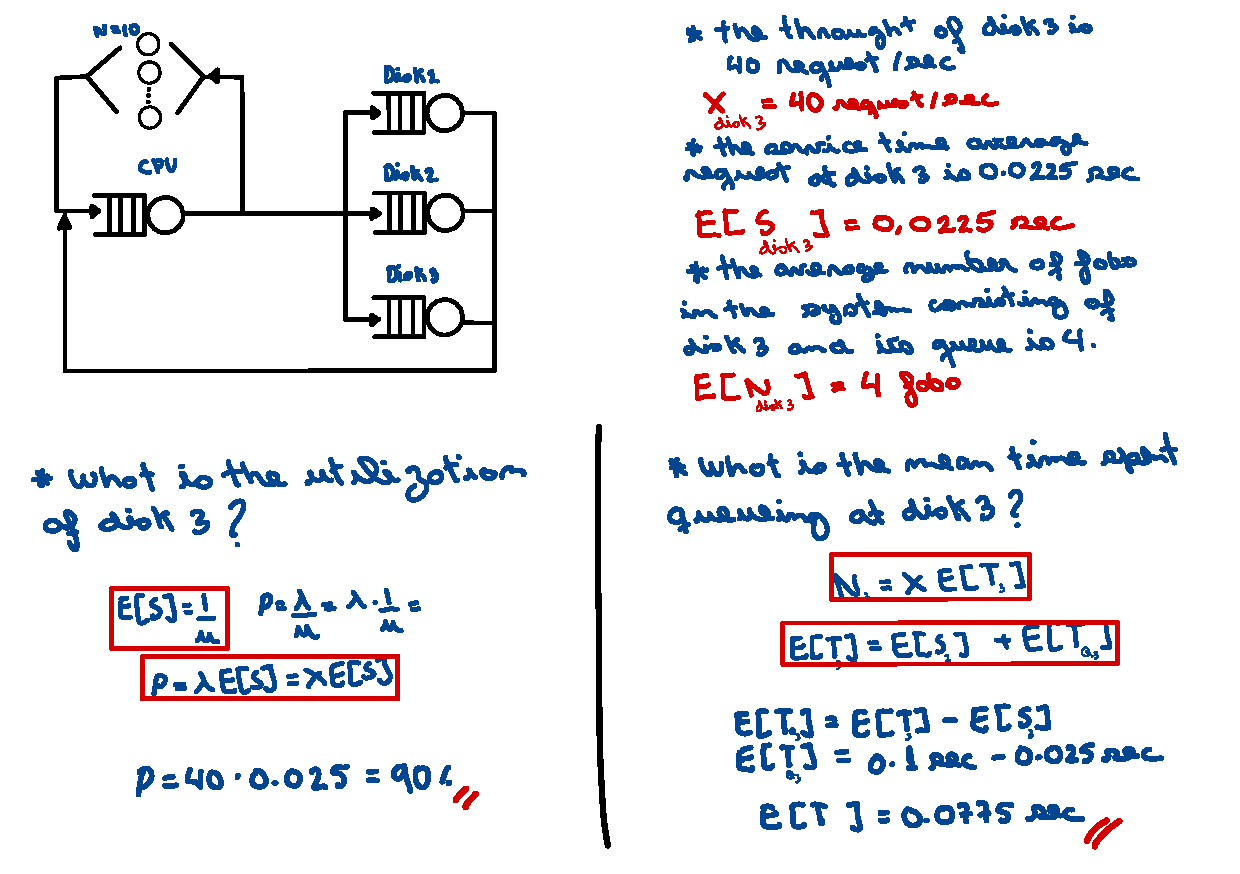
\includegraphics[width=0.95\textwidth]{slides/figures/little_law_closed_example.pdf}
    \end{figure}
\end{frame}



\begin{frame}
    \frametitle{Little's Law: Example}
    \begin{figure}
        \centering
        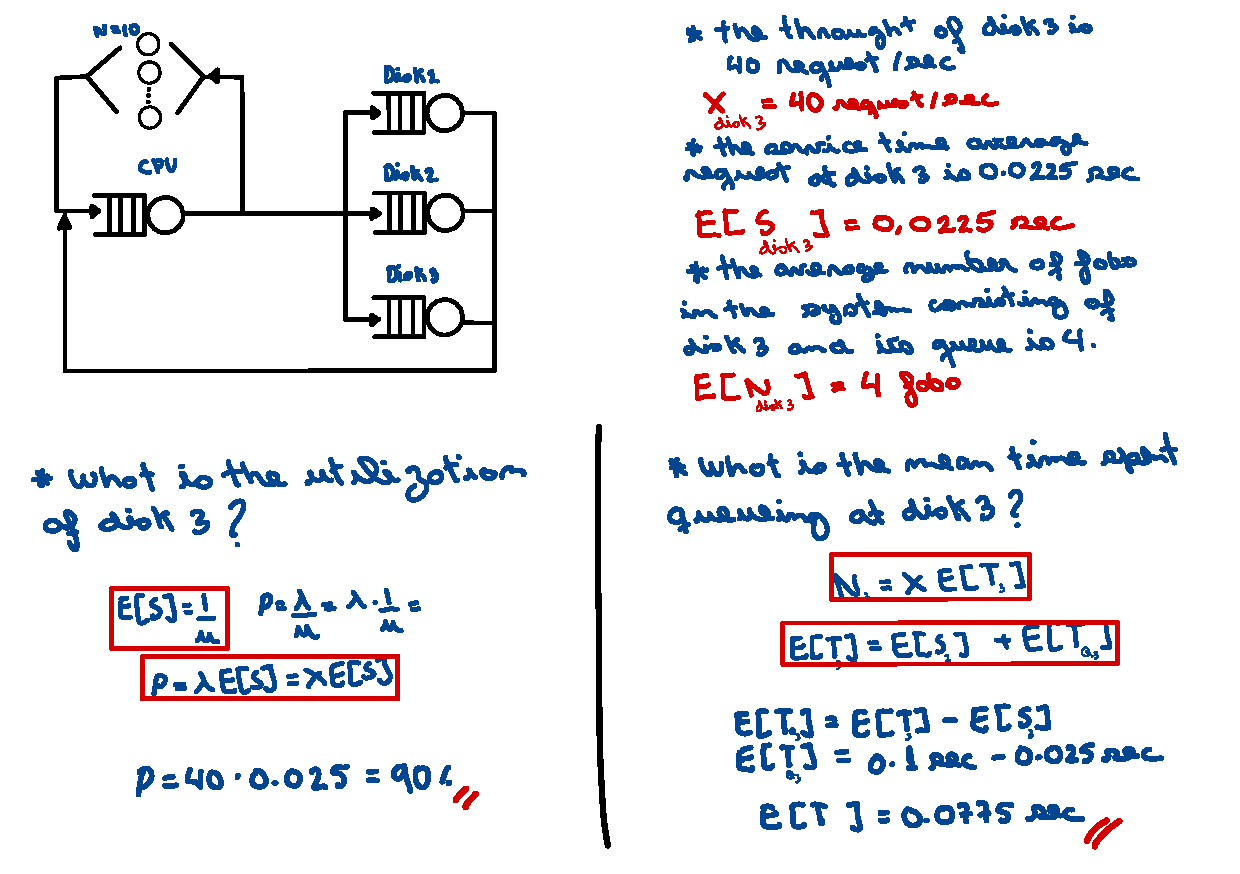
\includegraphics[width=0.95\textwidth]{slides/figures/little_law_closed_example.pdf}
    \end{figure}
\end{frame}


\subsection{Birth and Death Process}


\begin{frame}
    \frametitle{Markov Process}
    \begin{itemize}
        \item Queues can be modeled as a Markov Process;

        \item The time spent by a job in such queue is a Markov Process;

        \item The number of jobs in the queue is a Markov Process;
    \end{itemize}
\end{frame}



\begin{frame}
    \frametitle{Birth and Death Process: Balance Equation}
    \begin{figure}
        \centering
        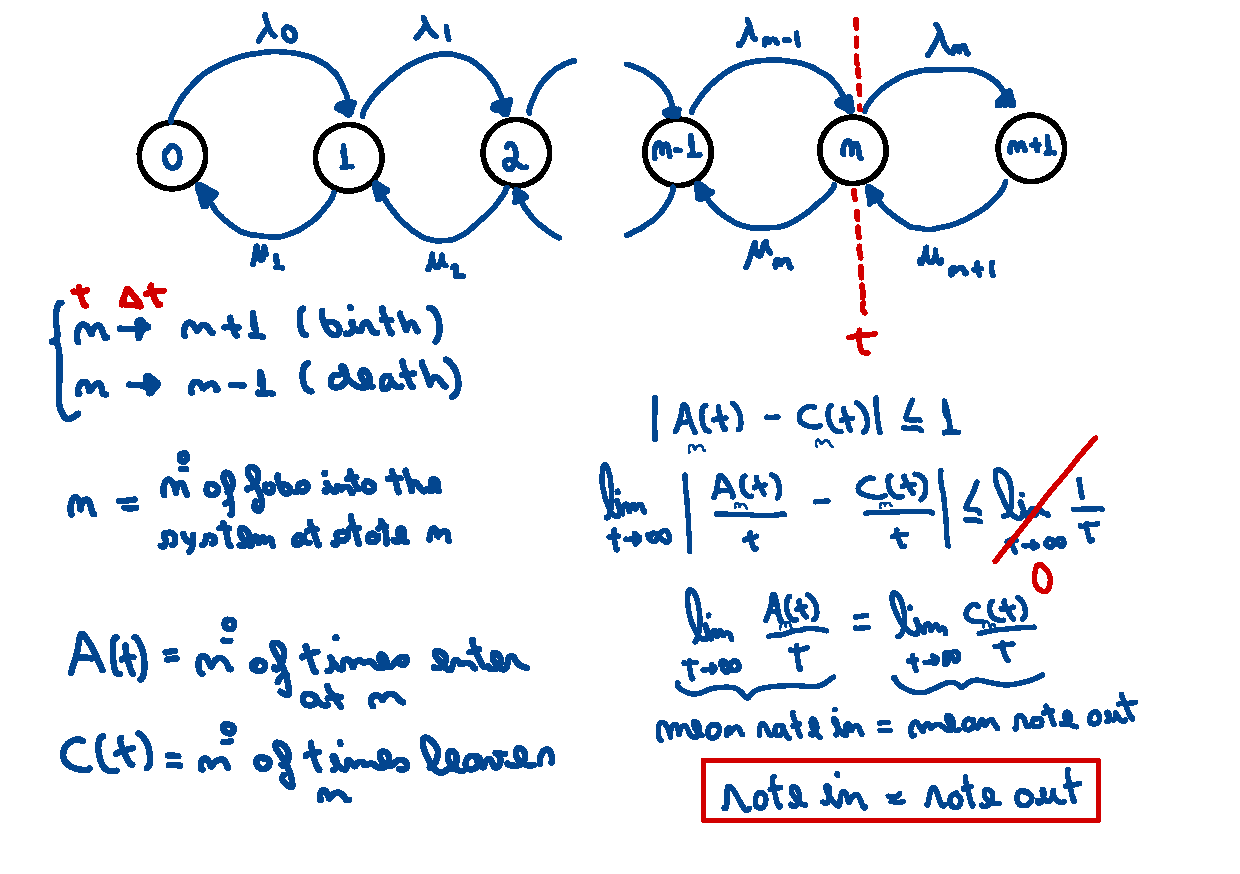
\includegraphics[width=0.95\textwidth]{slides/figures/balance_equation_proof.pdf}
    \end{figure}
\end{frame}


\begin{frame}
    \frametitle{Birth and Death Process}
    \begin{figure}
        \centering
        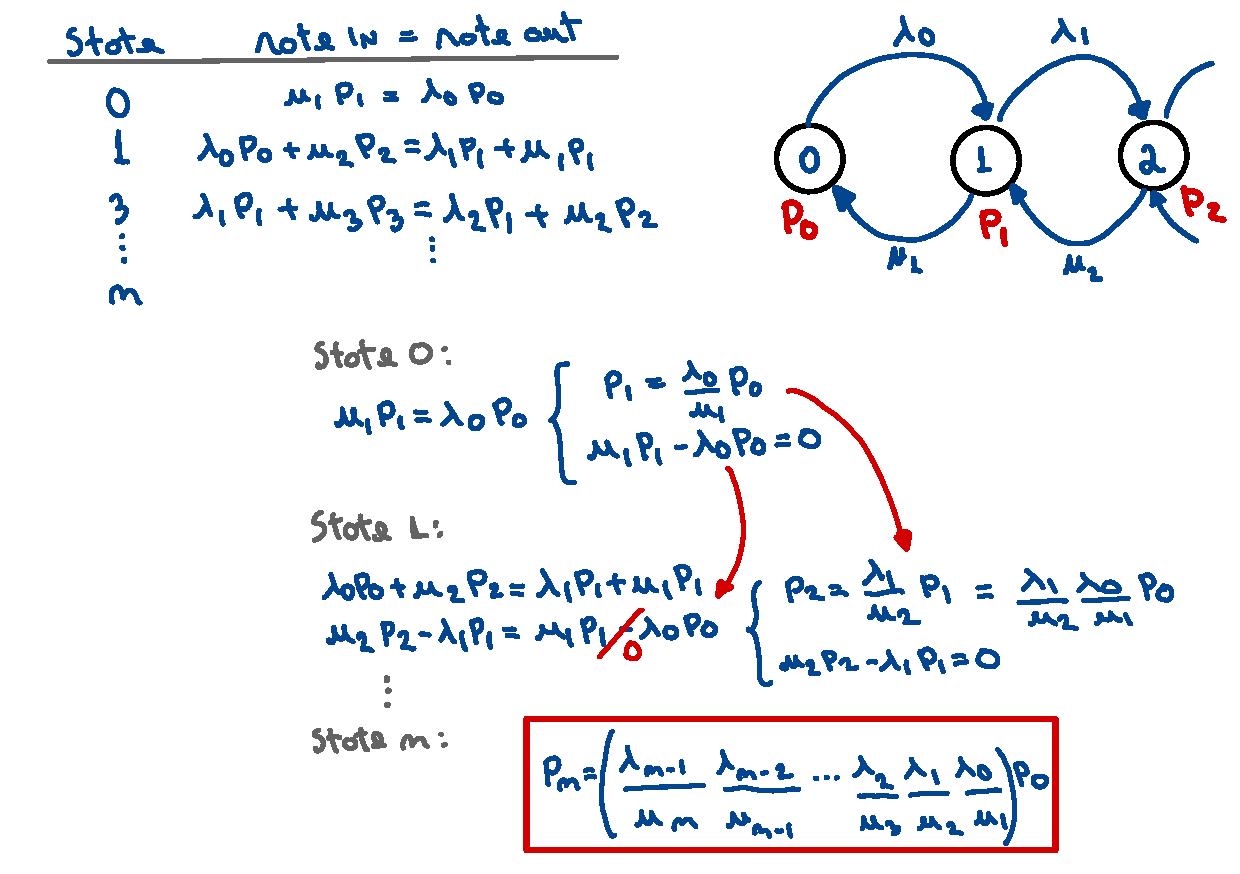
\includegraphics[width=0.95\textwidth]{slides/figures/balance_equation_prob_n.pdf}
    \end{figure}
\end{frame}


\begin{frame}
    \frametitle{Birth and Death Process}
    \begin{itemize}

        \item $P_n$ is given by

        $$P_n = \frac{\lambda_{n-1}\lambda_{n-2}...\lambda_{1}\lambda_{0}}{\mu_{n}\mu_{n-1}...\mu_{2}\mu_{1}}P_0$$

        \item Since $\lambda$ and $\mu$ are independent of the state, so we can rewrite $P_n$ as 

        $$P_n = \left(\frac{\lambda}{\mu}\right)P_0 \Rightarrow {\color{red}P_n = \rho^n P_0}$$

        \item It is important to remember that the sum of all probabilities is equal to 1

        $$\sum_{n=0}^{\infty}\rho^n P_0 = 1$$

    \end{itemize}
\end{frame}

\begin{frame}
    \frametitle{Simple Queue Expressions (1)}
    Let's derive the expected number of jobs in the system in 
    terms of $\lambda$ and $\mu$.

    \begin{figure}
        \centering
        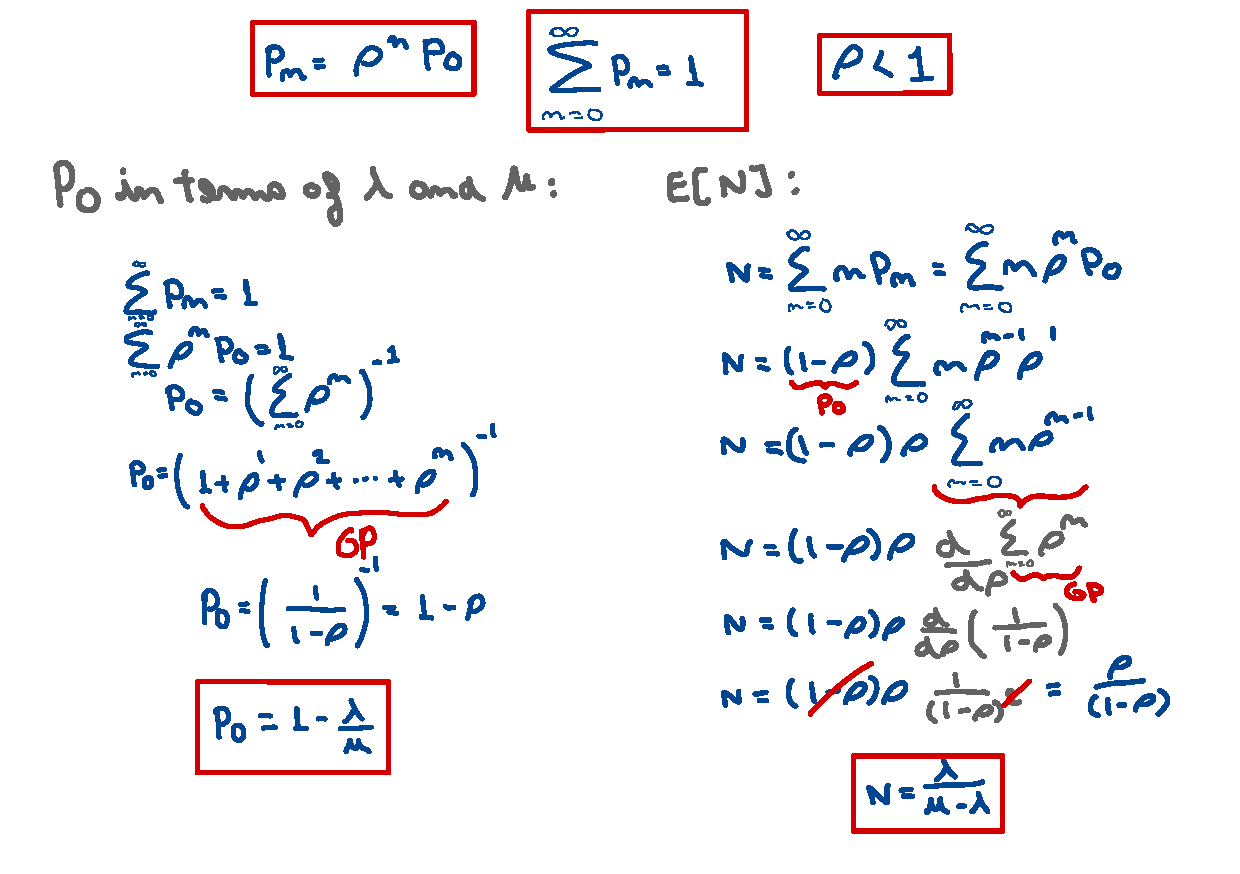
\includegraphics[width=0.8\textwidth]{slides/figures/simple_queue_expected_n.pdf}
    \end{figure}
\end{frame}


\begin{frame}
    \frametitle{Simple Queue Expressions (2)}
    Let's derive the expected number of jobs in the queue, expected time in the system and
    expected time in the queue in terms of $\lambda$ and $\mu$.

    \begin{figure}
        \centering
        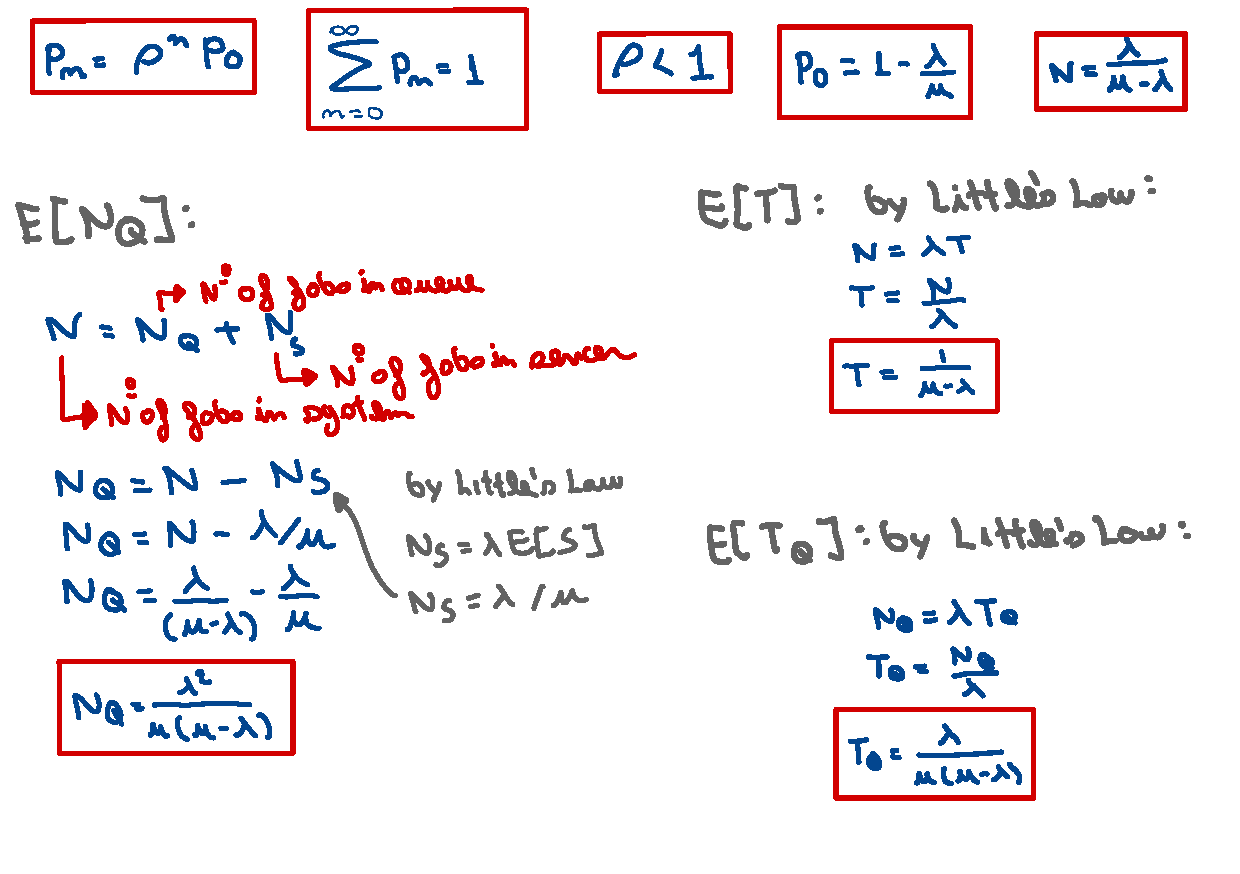
\includegraphics[width=0.8\textwidth]{slides/figures/simple_queue_expected_time.pdf}
    \end{figure}
\end{frame}

\subsection{Kendall's Notation}

\begin{frame}
    \frametitle{Kendall's Notation}
    \begin{itemize}
        \item It is important to note that these expressions were derived for 
        a simple queue model;

        \item Depends of the type of the queue, these expressions will change;

        \item Let's introduce the Kendall's notations used to describe and classify a queueing node (system).
    
    \end{itemize}

\end{frame}

\begin{frame}
    \frametitle{Kendall's Notation A/S/m(/B/K/SD)}
    Six parameters in shorthand.
    \begin{itemize}
        \item A: Arrival process;
        \item S: Service time distribution;
        \item m: Number of servers;
        \item B: Number of buffers or system capacity (infinity if not specified);
        \item k: Population size (infinite);
        \item SD: Service discipline (FCFS).
    \end{itemize}
\end{frame}


\begin{frame}
    \frametitle{Kendall's Notation: Distributions}
    \begin{itemize}
        \item M: Stands for "Markovian", implying exponential distribution for
        service times or inter-arrival times. "M" for "memoryless";
        \item D: Deterministic (e.g., fixed constant);
        \item $E_k$: Erlang with parameter $k$;
        \item $H_k$: Hyperexponential with parameter $k$;
        \item G: General (anything)
    \end{itemize}
\end{frame}



\begin{frame}
    \frametitle{Kendall's Notation: Examples}
    \begin{figure}
        \centering
        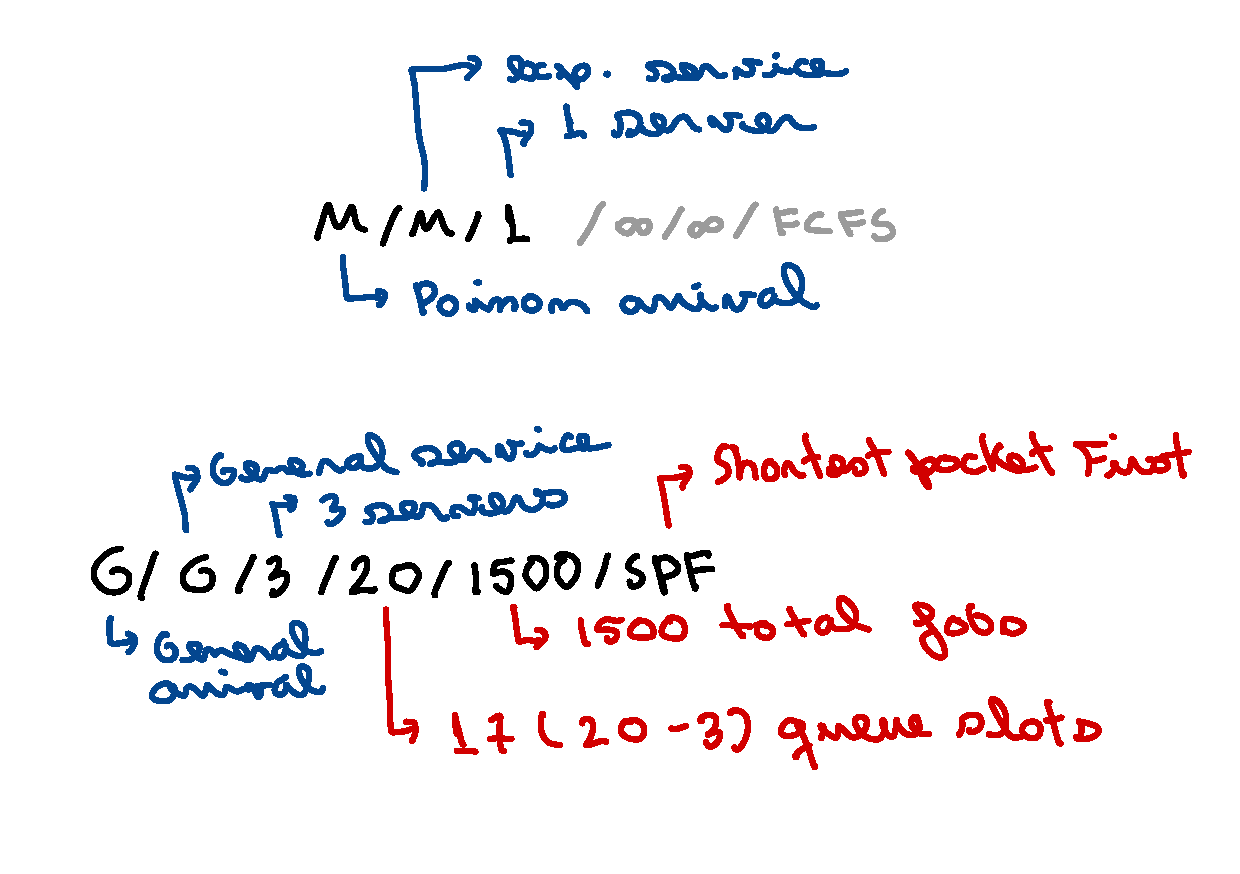
\includegraphics[width=0.95\textwidth]{slides/figures/kendall_examples.pdf}
    \end{figure}
\end{frame}


\subsection{Queue Models}

\begin{frame}
    \frametitle{The M/M/1 Queue (a.k.a Simple Network): Review}
    \begin{itemize}

        %\item $P_0$ in terms of $\lambda$ and $\mu$:
        %$$P_0 = 1 - \frac{\lambda}{\mu}$$

        \item Expected number of jobs in the system:
        $$E[N] = \frac{\lambda}{(\mu - \lambda)}$$

        \item Expected number of jobs in the queue:

        $$E[N_Q] = \frac{\lambda^2}{\mu(\mu-\lambda)}$$

        \item Expected job time in the system:

        $$E[T_Q] = \frac{\lambda}{\mu(\mu-\lambda)}$$

        \item Expected job time in the queue:

        $$E[T] = \frac{1}{\mu-\lambda}$$
    \end{itemize}
\end{frame}

\begin{frame}
    \frametitle{The M/M/c Queue}
    \begin{figure}
        \centering
        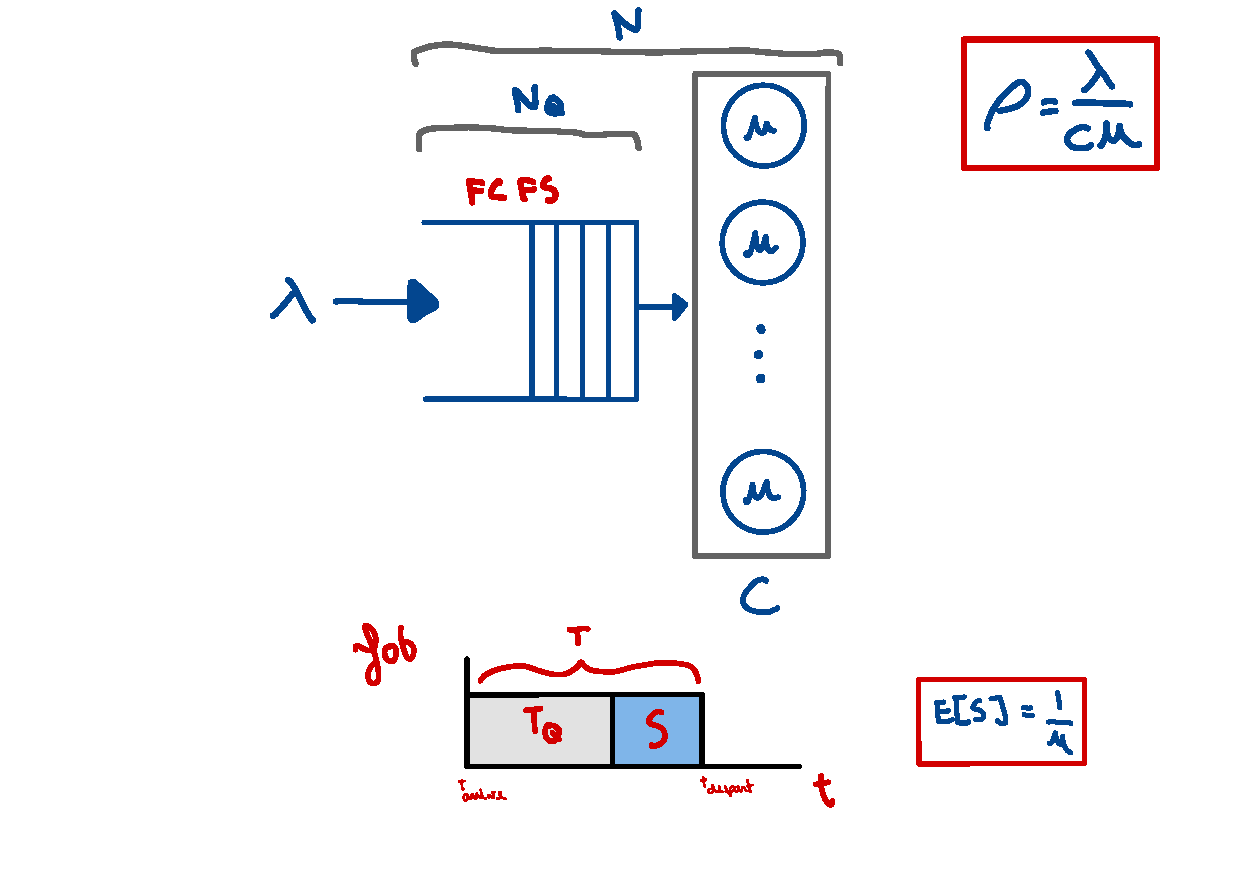
\includegraphics[width=0.95\textwidth]{slides/figures/mmc_queue.pdf}
    \end{figure}
\end{frame}

\begin{frame}
    \frametitle{The M/M/c Expressions (1)}
    \begin{figure}
        \centering
        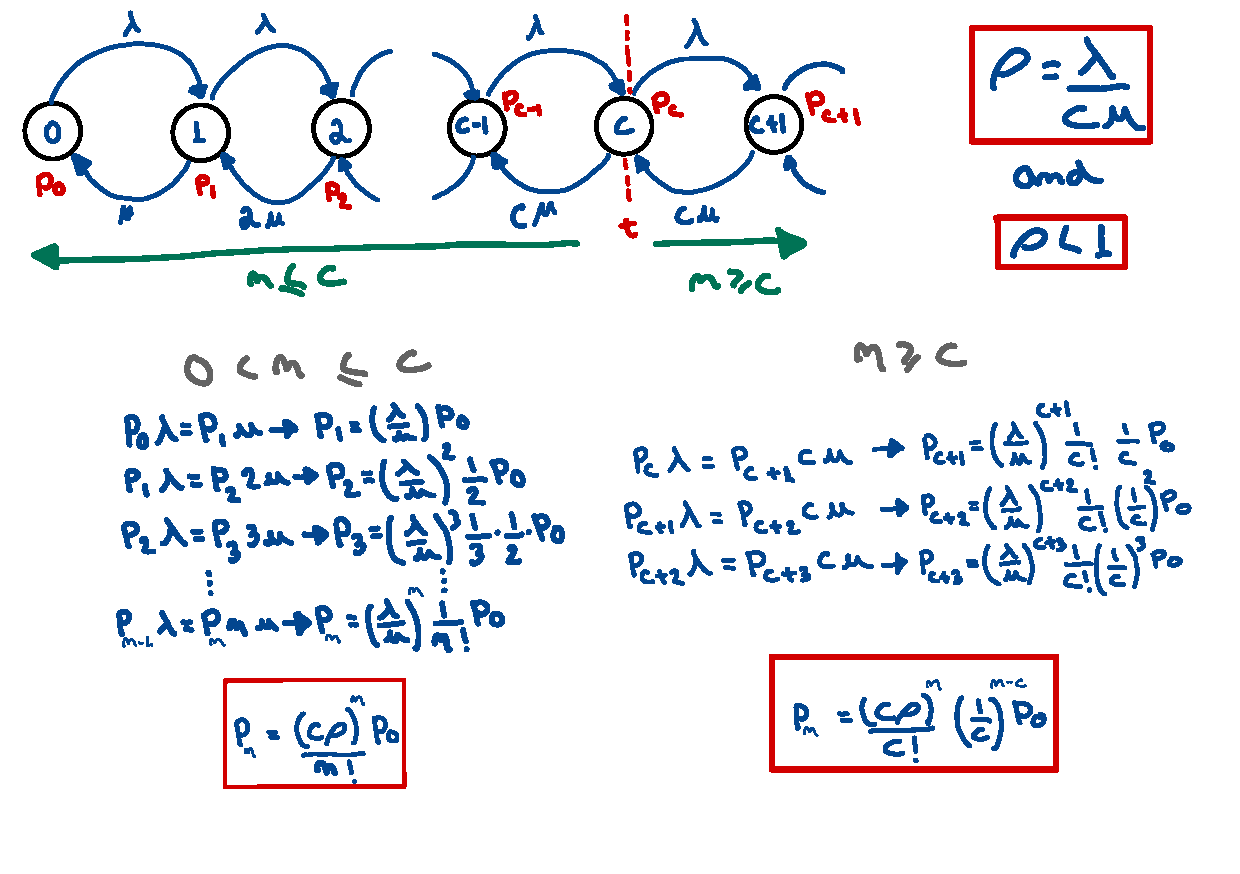
\includegraphics[width=0.95\textwidth]{slides/figures/mmc_equations_one.pdf}
    \end{figure}
\end{frame}

\begin{frame}
    \frametitle{The M/M/c Expressions (2)}
    \begin{figure}
        \centering
        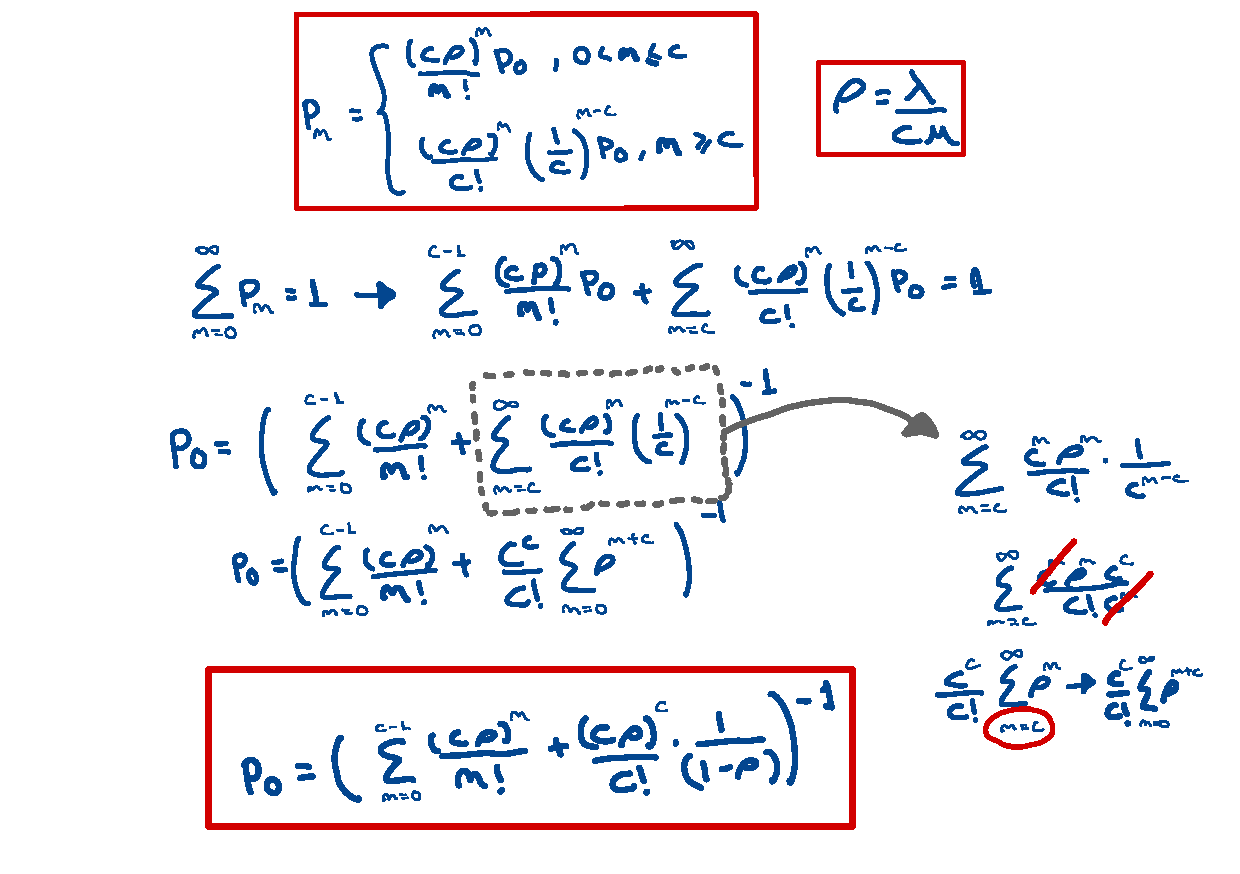
\includegraphics[width=0.95\textwidth]{slides/figures/mmc_equations_two.pdf}
    \end{figure}
\end{frame}


\begin{frame}
    \frametitle{The M/M/c: Performance Measures ($N_Q$)}

        It is clearly easier to begin by computing the expected queue length ($N_Q$) since only $P_n$'s involved
        are those for which $n\leq c$.

        $$N_Q = \sum_{n=c}^{\infty}(n-c)P_n$$

        with 

        $$P_n = \frac{(\rho c)^n}{c!c^{n-c}}P_0~~~\text{for $n\leq c$}$$

        which implies that

        $$N_Q = \sum_{n=c}^{\infty} \frac{n}{c^{n-c}c!}(\rho c)^{n}P_0 - \sum_{n=c}^{\infty} \frac{c}{c^{n-c}c!}(\rho c)^{n}P_0$$

\end{frame}


\begin{frame}
    \frametitle{The M/M/c: Performance Measures ($N_Q$)}

    After some algebric manipulations\footnote{pags 421--422 from Probability, Markov chains, queues, and 
    simulation book} we have
    $$N_Q = \frac{(\lambda/\mu)^c\lambda\mu}{(c-1)!(c\mu - \lambda)^2}P_0$$

    The probability than an arriving job is forced to wait is given by:
    $$P(queueing) = \sum_{n=c}^{\infty}P_n = \frac{(c\rho)^c}{(c!(1-\rho))}P_0 = C(c,\lambda/\rho)$$
\end{frame}


\begin{frame}
    \frametitle{The M/M/c: Performance Measures ($N$,$T$ and $T_Q$)}

    Having computed $N_Q$, we are now in position to find other performance measures.
    From Little's Law we can derive:

    \begin{itemize}
        \item Expected time of the job in the queue ($T_Q$):
        $$N_Q = \lambda T_Q$$
        \item Expected time of the job in the system ($T$):
        $$T = T_Q + E[S] = T_Q + 1/\mu$$
        \item Expected size of jobs in the system ($N$):
        $$N = \lambda T$$
    \end{itemize}
\end{frame}



\begin{frame}
    \frametitle{The M/M/c: Performance Measures}
    \begin{itemize}
        \item Expected number of jobs in the queue ($N_Q$):
        $$N_Q = \frac{(\lambda/\mu)^c\lambda\mu}{(c-1)!(c\mu - \lambda)^2}P_0$$
        \item Expected time of the job in the queue ($T_Q$):
        $$T_Q = \frac{C(c,\lambda/\mu)}{c\mu - \lambda}$$
        \item Expected time of the job in the system ($T$):
        $$T = \frac{C(c,\lambda/\mu)}{c\mu-\lambda} + \frac{1}{\mu}$$
        \item Expected size of jobs in the system ($N$):
        $$N = \frac{\lambda C(c, \lambda/\mu)}{c\mu-\lambda} + \frac{\lambda}{\mu}$$
    \end{itemize}
\end{frame}




\begin{frame}
    \frametitle{Finity Capacity Systems: The M/M/c/K Queue}
    \begin{figure}
        \centering
        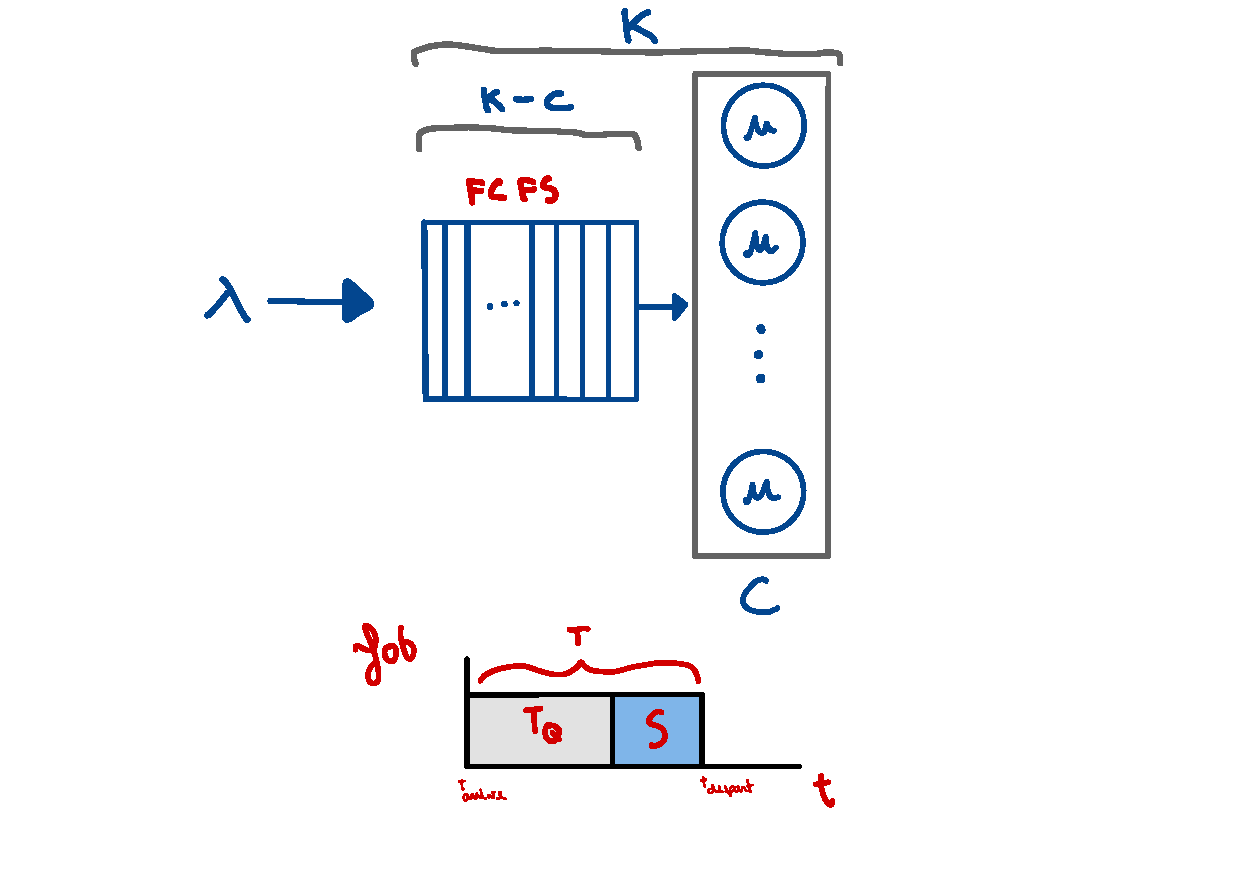
\includegraphics[width=0.95\textwidth]{slides/figures/mmck_queue.pdf}
    \end{figure}
\end{frame}


\begin{frame}
    \frametitle{The M/M/c/K Expressions (1)}
    \begin{figure}
        \centering
        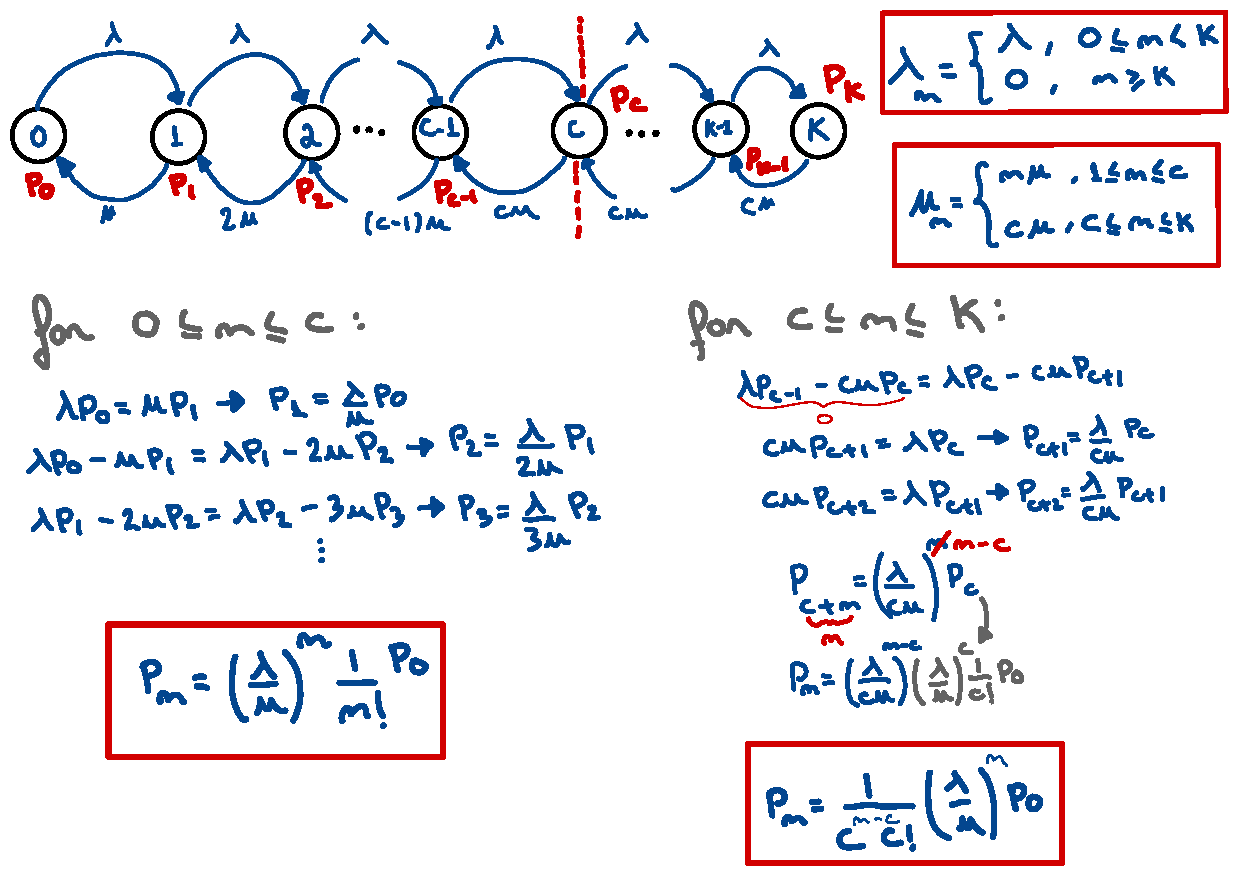
\includegraphics[width=0.95\textwidth]{slides/figures/mmck_equations_one.pdf}
    \end{figure}
\end{frame}


\begin{frame}
    \frametitle{The M/M/c/K Expressions (2)}
    In the end, we can use these expressions to derive the performance measures like $N$, $N_Q$, $T$ and $T_Q$.
    \begin{figure}
        \centering
        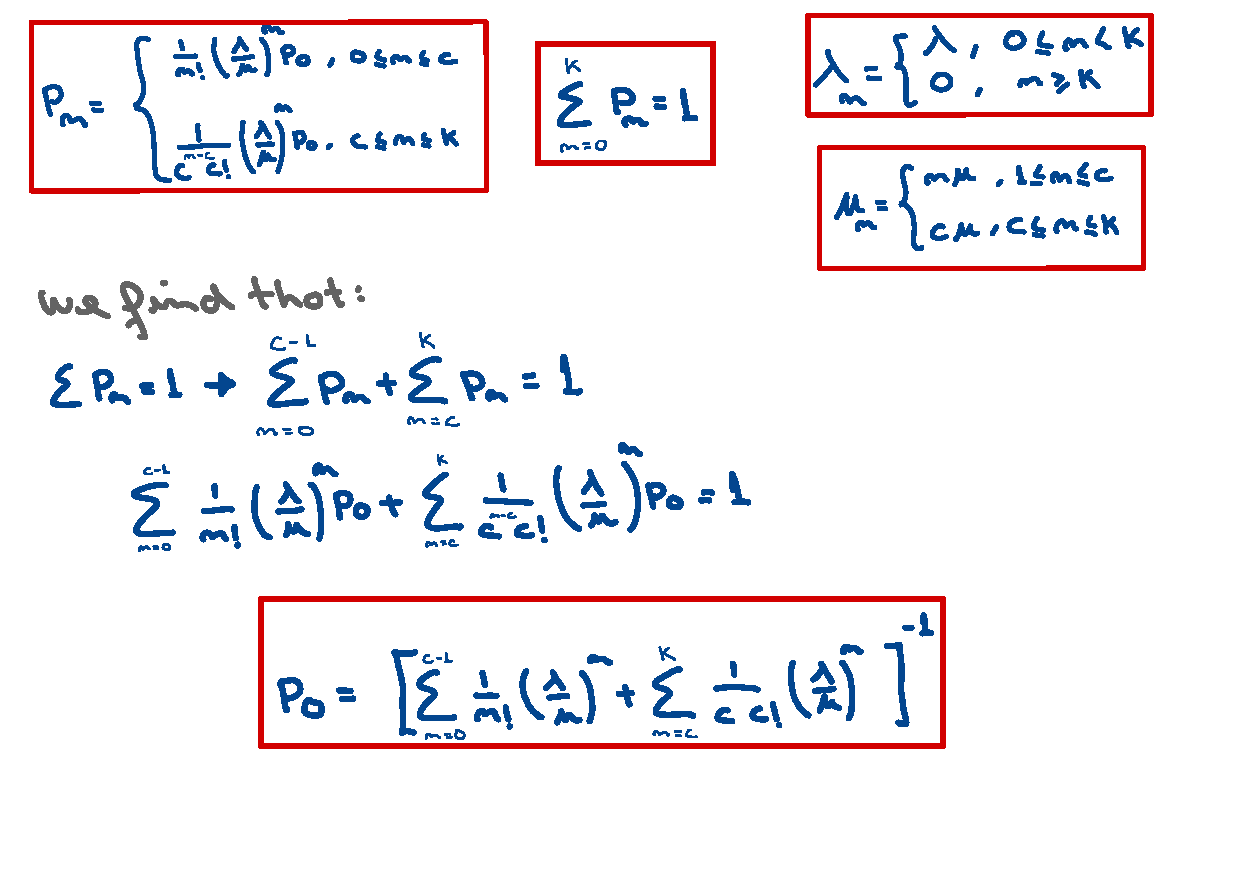
\includegraphics[width=0.95\textwidth]{slides/figures/mmck_equations_two.pdf}
    \end{figure}
\end{frame}



\section{Scheduling Policies}

\begin{frame}
    \frametitle{Scheduling Policies}

    There are several criteria for invoking the best scheduling policies for a system:

    \begin{itemize}
        \item \textbf{CPU Utilization:} Reduces the strain on the CPU and manages the percentage of time the CPU is busy.
        \item \textbf{Throughput ($X$):} Increases the number of processes (jobs) completed in a given time frame. 
        \item \textbf{Wait Time ($T_Q$):} Reduces the waiting time of a process (job).
        \item \textbf{Response Time:} Minimizes the time a user has to wait for a process to run;
        \item \textbf{Turnaround Time ($T$):} Total time a process (job) takes to run, from start to finish (includes all waiting time)
    \end{itemize}
\end{frame}




\begin{frame}
    \frametitle{Scheduling Policies}

    There are six popular process scheduling algorithms which we are going to discuss

    \begin{itemize}

        \item First-Come, First-Served (FCFS) Scheduling
        \item Shortest-Job-Next (SJN) Scheduling
        \item Priority Scheduling
        \item Shortest Remaining Time
        \item Round Robin(RR) Scheduling
        \item Multiple-Level Queues Scheduling

    \end{itemize}

    These algorithms are either non-preemptive or preemptive.

\end{frame}




\begin{frame}
    \frametitle{Scheduling Policies}
    \begin{itemize}

        \item \textbf{Non-Preemptive priorities:} A job being served cannot be ejected back 
        into the queue to leave place for a job with higher priority;

        \item \textbf{Preemptive priorities:} A job of lower priority that is being served will 
        be thrown back into the queue to leave room for a higher priority job.

    \end{itemize}
\end{frame}



\begin{frame}
    \frametitle{First-Come-First-Served (FCFS)}

    This is the real-life example. The person who arrives first in the queue first buys the ticket and then the next one. 
    \begin{itemize}

        \item Non-preemptive algorithm;

        \item Average Waiting Time is not optimal;

        \item Cannot utilize resources in parallel;

    \end{itemize}
\end{frame}



\begin{frame}
    \frametitle{First-Come-First-Served (FCFS)}

    Burst Time (BT) refers to the time required by a process (or job) for its execution. 
    \begin{figure}
        \centering
        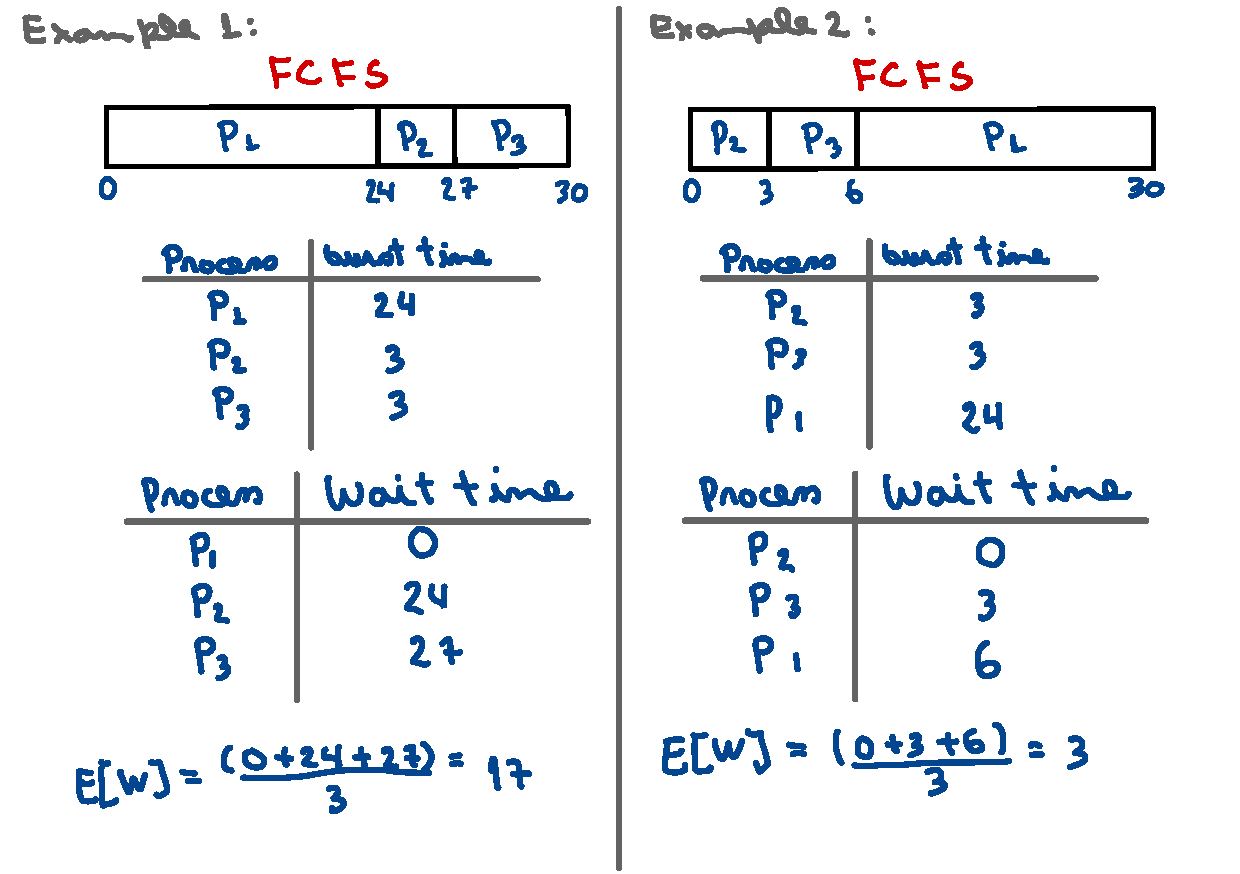
\includegraphics[width=0.85\textwidth]{slides/figures/fcfs_example.pdf}
    \end{figure}
\end{frame}

\begin{frame}
    \frametitle{Shortest Job First (SJF)}

    \begin{itemize}
        \item Non-preemptive and preemptive algorithm;
        \item Optimal average Waiting Time;
        \item Cannot utilize resources in parallel;
    \end{itemize}
\end{frame}


\begin{frame}
    \frametitle{Shortest Job First (SJF) Scheduling}
    \begin{figure}
        \centering
        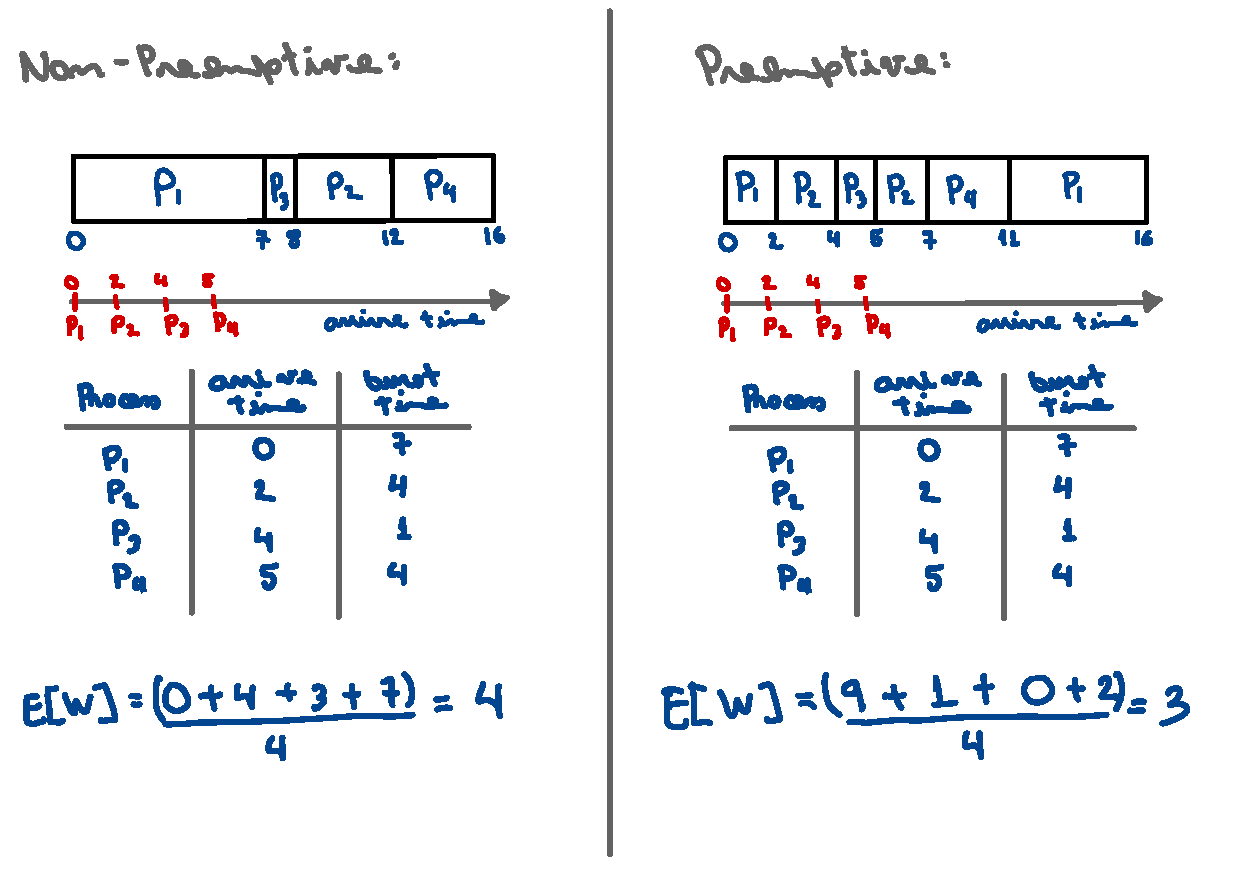
\includegraphics[width=0.85\textwidth]{slides/figures/sjf_example.pdf}
    \end{figure}
\end{frame}

\begin{frame}
    \frametitle{Priority Scheduling}

    Priority Scheduling is a process scheduling algorithm based on priority 
    where the scheduler selects tasks according to priority.

    \begin{itemize}
        \item Each process has a priority (integer number);
        \item Non-preemptive and preemptive algorithm;
        \item SJF is a priority scheduling where the priority is the burst time;
    \end{itemize}

    {\color{red}Stagnation:} 
    \begin{itemize}
        \item Problem: processes with low priority can never be executed;
        \item Solution: as time passes, process priority increases
    \end{itemize}

\end{frame}





\begin{frame}
    \frametitle{Round Robin (RR) Scheduling}

    
    \begin{itemize}
        \item Each process is allocated a small unit of CPU time (quantum).
        \item Time-sharing;
        \item Is a pre-emptive algorithm as the scheduler forces the process out of the CPU once the time quota expires.
        and added into the end of the queue.
        \item It is a real time algorithm which responds to the event within a specific time limit.
    \end{itemize}


\end{frame}

\begin{frame}
    \frametitle{Round Robin (RR) Scheduling}
    \begin{figure}
        \centering
        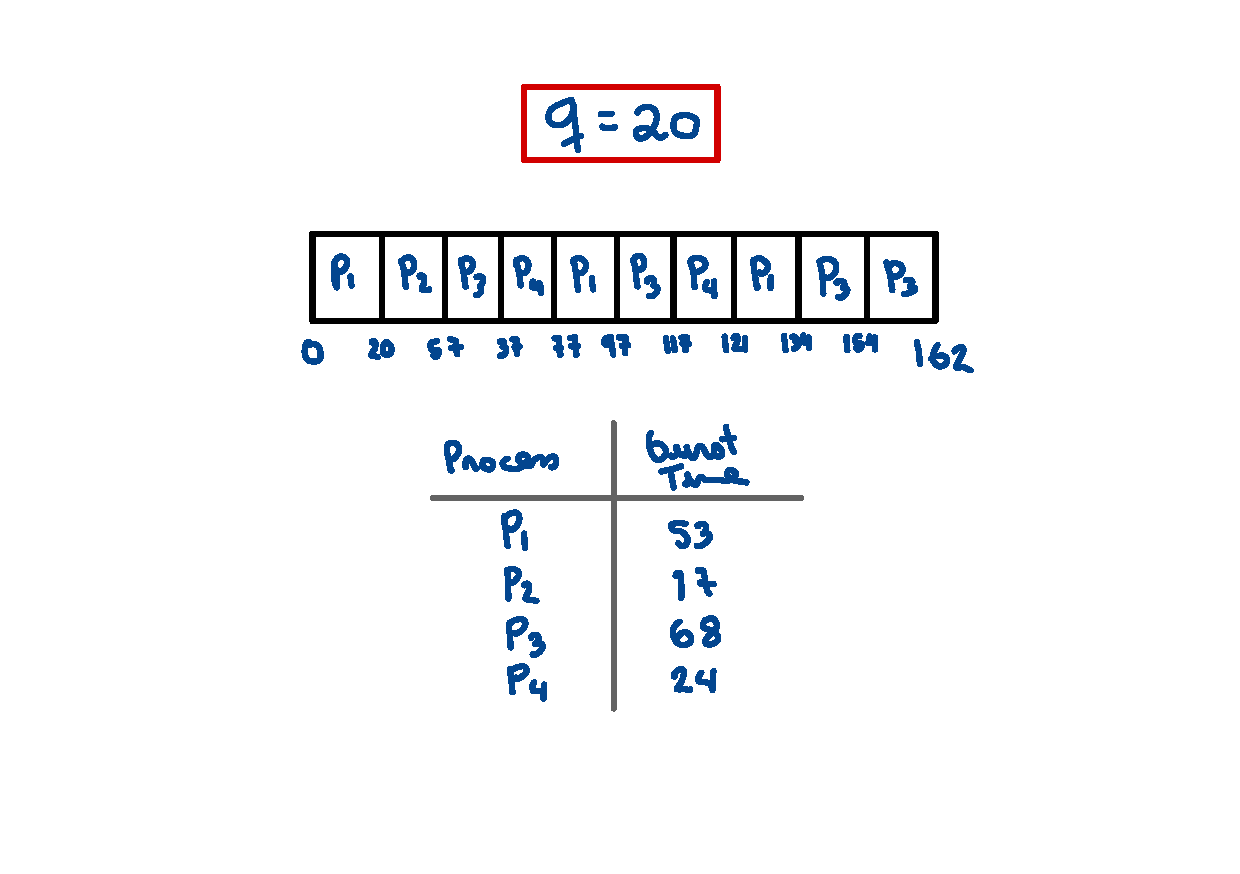
\includegraphics[width=0.95\textwidth]{slides/figures/round_robin_example.pdf}
    \end{figure}
\end{frame}



\begin{frame}
    \frametitle{Multilevel Queue Scheduling}
    \begin{itemize}

        \item is a queue with a predefined number of levels. Items get assigned to a particular level at 
        insert (using some predefined algorithm), and thus cannot be moved to another level (unlike in the multilevel feedback queue)

        \item Low scheduling overhead.

        \item Apply different scheduling methods to distinct processes.

        \item Some processes may face starvation as higher priority queues are never becoming empty.

    \end{itemize}
\end{frame}


\begin{frame}
    \frametitle{Multilevel Queue Scheduling}
    \begin{figure}
        \centering
        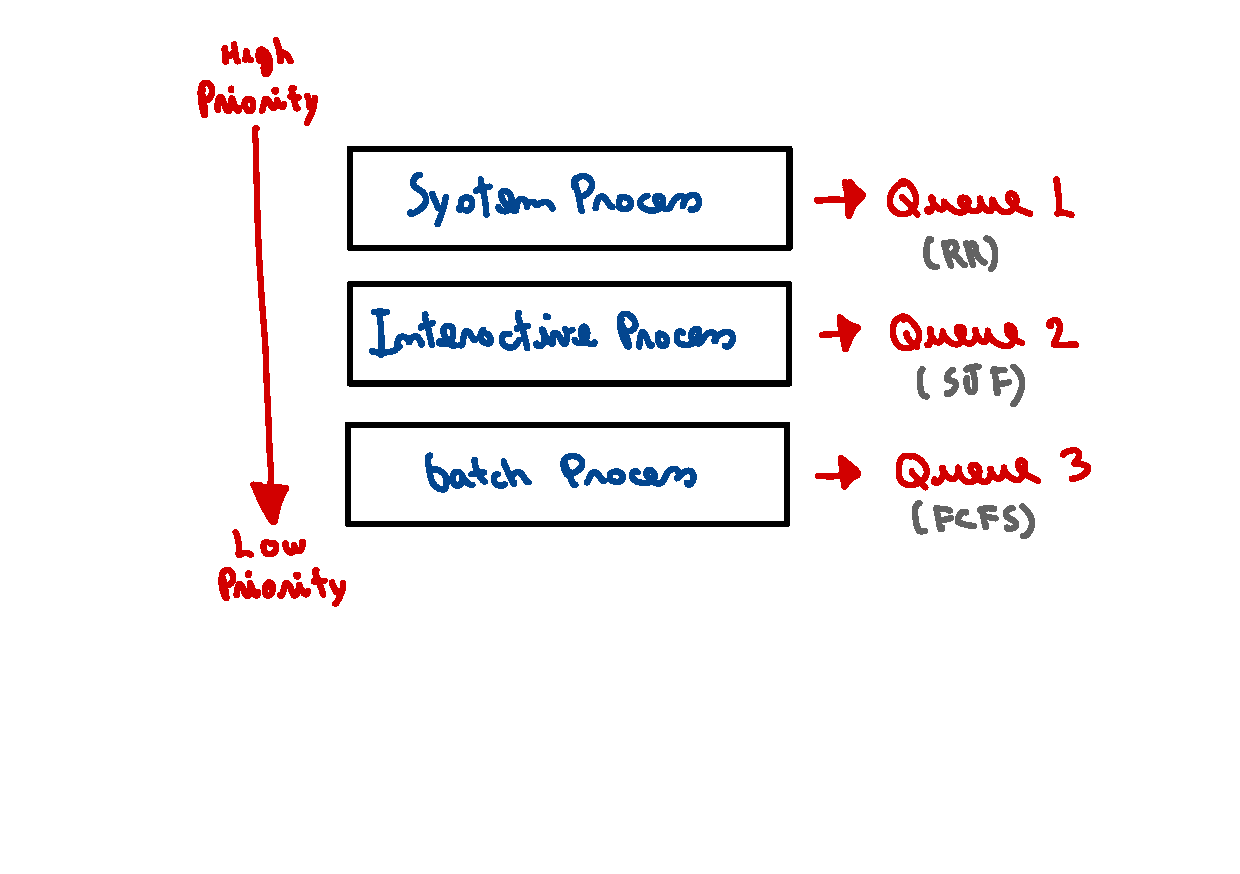
\includegraphics[width=0.95\textwidth]{slides/figures/mqs_example.pdf}
    \end{figure}
\end{frame}